\documentclass[12pt,a4paper,english]{article}
\usepackage[backend=biber]{biblatex}
\usepackage{float}
\usepackage{circuitikz}
\usepackage{caption}
\usepackage{graphicx}
\usepackage{epstopdf}
\usepackage{amsmath}
\usepackage{amssymb}
\usepackage{listings}
\usepackage{empheq}

\lstset{
basicstyle=\small\ttfamily,
columns=flexible,
breaklines=true,
showstringspaces=false,
frame=single
}

\setlength{\jot}{2ex}

\newcommand{\degree}[1]{\relax\ifmmode#1^\circ\else$#1^\circ$\fi}
\newcommand{\abs}[1]{\lvert#1\rvert}
\newcommand{\polar}[2]{#1 \angle \degree{#2}}
\newcommand{\db}[1]{\relax\ifmmode{#1\,\text{dB}}\else{#1 dB}\fi}
\newcommand{\dbw}[1]{\relax\ifmmode{#1\,\text{dBW}}\else{#1 dBW}\fi}
\newcommand{\dbm}[1]{\relax\ifmmode{#1\,\text{dBm}}\else{#1 dBm}\fi}
\newcommand{\logten}[1]{\relax\ifmmode{\log_{10}\left(#1\right)}\else{$\log_{10}\left(#1\right)$}\fi}
\newcommand{\boxedeq}[3]{\begin{empheq}[box={\fboxsep=6pt\fbox}]{#3}\label{#1}#2\end{empheq}}
\newcommand{\sci}[2]{\ifmmode{#1 \times 10^{#2}}\else{$#1 \times 10^{#2}$}\fi}
\newcommand{\ohm}{\ifmmode{\Omega}\else{$\Omega$}\fi}
% \newenvironment{eqbox}[1][align]{%
% \begin{empheq}[box={\fboxsep=6pt\fbox}]{#1}
% }{\end{empheq}}

\newenvironment{eqbox}[1][gather*]
{
  \empheq[box={\fboxsep=6pt\fbox}]{#1}
}
{
  \endempheq
}

\title{Temperature Buffer Design Notes}
\author{Alex Hansen\\ajhansen@usf.edu\\(727) 465-4797}
\date{\today}

%\addbibresource{postlab01.bib}

\usepackage{titlesec}

\titleformat{\section}
  {\normalfont\Large\bfseries}   % The style of the section title
  {}                             % a prefix
  {0pt}                          % How much space exists between the prefix and the title
  {}    % How the section is represented

\titleformat{\subsection}
  {\normalfont\bfseries}
  {}
  {0pt}
  {}

\begin{document}

  \maketitle
  \thispagestyle{empty}
  \clearpage

  \section{Block Diagram}

  \begin{figure}[H]
     \centering
     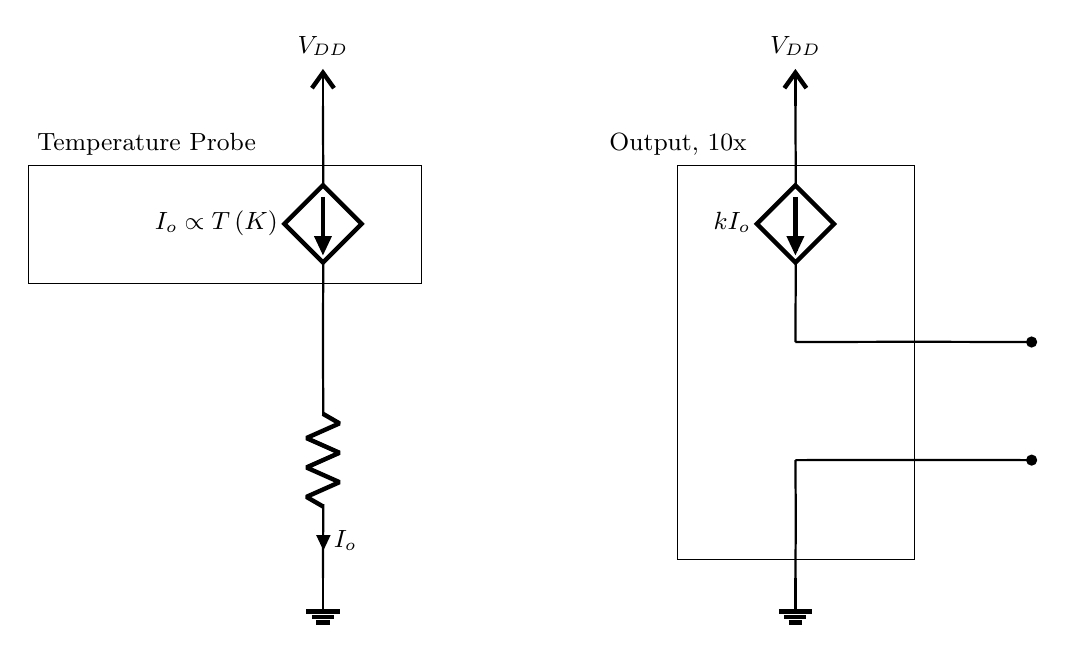
\begin{tikzpicture}
     [
     scale=1.5,
     every node/.style={font=\small},
     american voltages,
     american currents,
     american resistors
     ]
     \draw[color=black, thick]
     (10,10) node [vcc] {$V_{DD}$}
     (10,10) to [cI, l_=$I_o \propto T \, (K)$] (10,8)
     (10,8)  to [R, i=$I_o$] (10, 6)
     (10,6)  node [ground] {}
     (14,10)  node [vcc] {$V_{DD}$}
     (14,10)  to [cI, l_=$k I_o$] (14,8)
     (14,8) to [short, -*] (16,8)
     (14,7) to [short, -*] (16,7)
     (14,7) to [short] (14,6)
     (14,6) node [ground] {}
     ;
     \node[draw,minimum width=5cm,minimum height=1.5cm,anchor=north west,label={[xshift=-1.0cm]Temperature Probe}] at (7.5, 9.5) {};
     \node[draw,minimum width=3cm,minimum height=5cm,anchor=north west,label={[xshift=-1.5cm]Output, 10x}] at (13,9.5) {};
     \end{tikzpicture}
     \label{current_bus}
     \caption{The temperature probe produces an output current which is proportional to its temperature. The current
      buffer produces ten outputs, each of which reproduces the current output from the temperature sensor. The benefit
      of this design is that any number of output circuits (between one and ten) may be connected to the buffer without
      interfering with the operation of any other circuit.}
   \end{figure}


\end{document}
